%% LyX 1.6.2 created this file.  For more info, see http://www.lyx.org/.
%% Do not edit unless you really know what you are doing.
\documentclass[12pt,french,a4paper]{article}
\usepackage[T1]{fontenc}
\usepackage[utf8]{inputenc}
\setcounter{secnumdepth}{2}
\setcounter{tocdepth}{2}
\usepackage{array}
\usepackage{graphicx}

\makeatletter

%%%%%%%%%%%%%%%%%%%%%%%%%%%%%% LyX specific LaTeX commands.
%% Special footnote code from the package 'stblftnt.sty'
%% Author: Robin Fairbairns -- Last revised Dec 13 1996
\let\SF@@footnote\footnote
\def\footnote{\ifx\protect\@typeset@protect
    \expandafter\SF@@footnote
  \else
    \expandafter\SF@gobble@opt
  \fi
}
\expandafter\def\csname SF@gobble@opt \endcsname{\@ifnextchar[%]
  \SF@gobble@twobracket
  \@gobble
}
\edef\SF@gobble@opt{\noexpand\protect
  \expandafter\noexpand\csname SF@gobble@opt \endcsname}
\def\SF@gobble@twobracket[#1]#2{}
%% Because html converters don't know tabularnewline
\providecommand{\tabularnewline}{\\}

%%%%%%%%%%%%%%%%%%%%%%%%%%%%%% User specified LaTeX commands.



\usepackage{hyperref}


%\usepackage{longtable}


\setlength{\headheight}{0cm}
\setlength{\headsep}{0cm}
\setlength{\topskip}{0cm}
\setlength{\topmargin}{-0.5cm}

\setlength{\parskip}{1.5ex}
\setlength{\parindent}{0cm}
\setlength{\oddsidemargin}{0cm}
\setlength{\textwidth}{16cm}
\setlength{\textheight}{27cm}

\newlength{\maximgwidth}
\setlength{\maximgwidth}{14cm}
\newcommand{\maximage}[1]{	
\begin{center}
\includegraphics[width=\maximgwidth]{#1} 
\end{center}
}
\newcommand{\hint}[1]{
\begin{center} 
\begin{tabular}{|rp{12cm}|} \hline
{\bf Astuce }:& #1\\	\hline
\end{tabular}
\marginpar{\Huge !} 
\end{center} 
}

\newcommand{\vym}{{\sc vym }}
\newcommand{\ra}{$\longrightarrow$}
\newcommand{\la}{$\longleftarrow$}
\newcommand{\ua}{$\uparrow$}
\newcommand{\da}{$\downarrow$}
\newcommand{\key}[1]{[#1]}

%\newenvironment{code}[1]{ \verbatim #1}{\endverbatim  }

\hypersetup{bookmarks, bookmarksopen,
  pdftitle={VYM - a tool for visual thinking },
  pdfauthor={Uwe Drechsel},    
  pdfsubject={map},
  pdfkeywords={map, tool},
  pdfpagemode={UseOutlines},                                 
  bookmarksopenlevel={1},   
  colorlinks={true},     
  linkcolor={blue},
  urlcolor={green},
  citecolor={red}} 

\makeatother

\usepackage{babel}
\addto\extrasfrench{\providecommand{\og}{\leavevmode\flqq~}\providecommand{\fg}{\ifdim\lastskip>\z@\unskip\fi~\frqq}}

\begin{document}

\title{
\includegraphics[width=8cm,bb = 0 0 200 100, draft, type=eps]{images/vym-logo-new.png}
\\
 VYM \\
 -- \\
View Your Mind\\
 {\small Version 1.12.0}\\
{\small (version française)}}


\author{\textcopyright Uwe Drechsel }

\maketitle
\newpage{}

\tableofcontents{}

\newpage{}


\section*{Remerciements}

Beaucoup de gens m'ont envoyé leurs impressions et leurs idées et
tout cela m'a aidé à faire \vym meilleur. Merci à tous !

Pour ce manuel, je remercie particulièrement :
\begin{itemize}
\item {\em Peter Adamson} pour un grand nombre de retours et pour la
relecture de mon anglais très imparfait,
\item L'équite du {\em AClibre (Academia y Conocimiento Libre)} en Colombie
pour leur traduction du manuel en espagnol : 


\begin{center}
\begin{tabular}{|p{7cm}|p{5.5cm}|}
\hline 
Encargado  & Actividad \tabularnewline
\hline 
\begin{itemize}
\item Vanessa Carolina Gutiérrez Sanchez 
\item Erika Tatiana Luque Melo 
\item Jeffrey Steve Borbón Sanabria 
\item John Edisson Ortiz Román 
\end{itemize}
 & \begin{itemize}
\item Traducciónl 
\item Revisión y correcciones varias 
\item Estructuración y exporte 
\item Revisión y correcciones varias 
\end{itemize}
\tabularnewline
\hline
\end{tabular}
\par\end{center}

\end{itemize}
\newpage{}


\section*{Note du traducteur}

Correspondances entre les mots de la version originale en anglais
et la version française. Certains mots trop spécifiques à \vym  ont
été gardés en anglais.


\subsection*{traduits}
\begin{description}
\item [{ancre}] \emph{anchor }
\item [{canevas}] \emph{layout }
\item [{carte}] \emph{map }
\item [{défaire/refaire}] \emph{undo/redo }
\item [{emoticon}] \emph{smiley }
\item [{escamotage}] \emph{folding }
\item [{fils}] \emph{child }
\item [{indicateur}] \emph{flag }
\item [{menu~de~contexte}] \emph{context menu} 
\item [{menu~des~préférences}] \emph{settings menu }
\item [{mode~modificateur}] \emph{modifier (CTRL) }
\item [{navigateur}] \emph{webbrowser }
\item [{onglets}] \emph{bookmark }
\item [{patrons}] \emph{frame }
\item [{titre}] \emph{heading }
\item [{signets}] \emph{bookmark }
\item [{sous-arbre}] \emph{jeu de branches en dessous}
\item [{barre~de~travail}] \emph{toolbars}
\end{description}

\subsection*{non traduits}
\begin{description}
\item [{mapeditor}] fenêtre d'édition de la carte 
\item [{mapcenter}] milieu du mapeditor 
\item [{noteeditor}] fenêtre d'édition des notes
\item 
\end{description}
\clearpage 


\section{Introduction}


\subsection{Qu'est-ce qu'une carte \vym ?}

Une carte \vym (on abrégera sous le nom de {\em carte}) est une
structure en forme d'arbre : \maximage{images/example1_fr.png}
De telles cartes peuvent être faites à la main sur une feuille de
papier ou en brouillon et aident à structurer vos pensées. Alors qu'une
structure en forme d'arbre comme sur l'image ci-dessus peut être tracée
à la main, \vym offre des possibilités supplémentaires.

\vym n'est pas un logiciel de dessin supplémentaire, mais un outil
pour mémoriser et modifier l'information de façon intuitive. Par exemple,
vous pouvez réorganiser des parties de la carte en appuyant sur une
touche ou ajouter des informations comme un email complet simplement
par un clic de souris.

Un fois que vous avez fini de rassembler et d'organiser vos idées
vous pouvez générer des sorties ---basées sur une {\em carte}---
sous divers formats incluant une présentation dans Open-Office.

\hint{Vous trouverez la carte ci-dessus et les autres en cliquant
:

\begin{center}
Help \ra Open vym examples 
\par\end{center}

dans la barre de menu.}


\subsection{Pourquoi utiliser des {\em cartes}? l'Espace, le Temps et votre
cerveau}


\subsubsection*{Espace}

Une {\em carte} peut concentrer un contenu très complexe sur un
petit espace comme une feuille de papier. Cela aide les deux côtés
de votre cerveau : le côté logique et le côté créatif (par exemple
en utilisant des dessins, des couleurs et des mots clé, souvent appelés
{\em ancres}. C'est une technique pour aider à organiser votre
façon de penser et stimuler votre créativité : cela vous aide en développant,
classant et mémorisant vos idées.


\subsubsection*{Temps}

Parce que vous utilisez des mots clé et des dessins, c'est plus rapide
que les bonnes vieilles \og notes \fg. Votre cerveau mémorise les
choses par association avec d'autres choses -- une {\em carte}
utilise ces connexions et stimule de nouvelles associations.


\subsubsection*{Votre cerveau}

En 1960 le professeur \textsc{Roger Sperry} découvre que les deux
hémisphères du cerveau humain s'occupent de domaines différents mais
{\em peuvent } faire les mêmes choses : 

\begin{center}
\begin{tabular}{|p{5.5cm}|p{5.5cm}|}
\hline 
Côté gauche  & Côté droit\tabularnewline
\hline 
\begin{itemize}
\item expression verbale et écrite,
\item nombres,
\item pensée logique, 
\item analyse et détails,
\item science,
\item pensée linéaire,
\item concept de temps.
\end{itemize}
 & \begin{itemize}
\item langage du corps, 
\item pensée visuelle, rêves éveillés,
\item intuition et émotion,
\item capacité de synthèse,
\item créativité,
\item art, musique, danse, 
\item pensée non linéaire, relation entre les choses,
\item conscience spatiale.
\end{itemize}
\tabularnewline
\hline
\end{tabular}
\par\end{center}

Dans notre société des sciences occidentales, nous avons appris à
relier principalement le côté gauche de notre cerveau, le côté \og
rationel \fg{}. Dans d'autres cultures, comme celles des vieilles
cultures indiennes ou d'autres \og vieilles\fg{} cultures, l'autre
côté (le droit) est plus important. Les {\em cartes} sont juste
un moyen de stimuler l'autre coté et d'utiliser les capacités supplémentaires
dont nous disposons tous.


\subsection{Où puis-je utiliser une {\em carte}?}

Voici quelques exemples et comment vous pouvez utiliser ces {\em
cartes} : 
\begin{itemize}
\item pour préparer des articles, des papiers, des livres, des discussions,
etc, 
\item pour trier des idées complexes, 
\item pour mémoriser des faits, des noms de personnes, du vocabulaire, etc, 
\item pour trier des emails, des fichiers et les signets de votre ordinateur, 
\item la préparation d'un exposé, 
\item des séances de remue-méninges pour résoudre des problèmes, 
\item pour enregistrer les tâches lors de l'organisation d'un projet. 
\end{itemize}

\subsection{Ce que vous ne pouvez pas faire avec une {\em carte}...}

Une {\em carte} tracée par quelqu'un montre la façon de penser
de son auteur. Elle n'a pas à être juste ou fausse, elle n'est pas
criticable.\og C'est ce que c'est \fg{}(\textsc{F.~Lehmann}).
L'outil est d'une très utile à son créateur mais d'un usage très limité
pour les autres.

Cependant quand un groupe s'investit dans la création d'une {\em
carte}, tout le groupe bénéficie de son utilisation. Quand un professeur
développe une {\em carte} avec un groupe d'élèves pendant un cours
ou quand un chef de projet recueille les informations d'un groupe
de spcialistes pour l'aider à \og{}{\em encarter}\fg{} les
tâches nécessaires pour réaliser ce projet.

%\section{Tutorials}
%TODO



\subsection{Ressources internet}

Un bon point de départ est d'en apprendre plus sur les {\em cartes
heuristiques} dans Wikipedia : 
\begin{itemize}
\item Anglais : \href{http://en.wikipedia.org/wiki/Mind_map}{http://en.wikipedia.org/wiki/Mind\_map} 
\item Allemand : \href{http://de.wikipedia.org/wiki/Mindmap}{http://de.wikipedia.org/wiki/Mindmap} 
\item Français : \href{http://fr.wikipedia.org/wiki/Mindmap}{http://fr.wikipedia.org/wiki/Mindmap}
(N.d.T.)
\end{itemize}

\section{Le Concept de \vym }

%TODO may add a general introduction here...



\subsection{La fenêtre principale et ses satellites}

\label{satellite} \vym vient avec plusieurs fenêtres, celle centrale
est le {\em mapeditor}. D'autres fenêtres, chacune avec une fonction
particulière peut être ouverte et installée à côté de la fenêtre principale%
\footnote{L'avantage des fenêtres séparées par rapport à une seule est une plus
grande flexibilité dans leur position. Par exemple j'utilise le {\em
noteeditor} \og derrière \fg{} le {\em mapeditor}. Sur Linux
mon gestionnaire de fenêtres (KDE) me permet de rentrer du texte dans
un petit coin visible du {\em noteeditor} sans cliquer dessus avec
la souris. Je positionne la souris sur la fenêtre pour y concentrer
le focus, un concept utile aussi lorsqu'on travaille avec \href{http://www.gimp.org}{http://www.gimp.org}. %
}. L'image en dessous montre le {\em mapeditor} avec le {\em noteeditor} souvent
utilisé : \maximage{images/windows_fr.png} La plupart du temps
vous travaillerez dans le {\em mapeditor} en ajoutant des nouvelles
branches, en les déplaçant et en les réarrangeant. Les diverses manières
de le faire sont expliquées dans \ref{mapeditor}. Vous pouvez enregistrer
des informations complémentaires par exemple le contenu d'un email
facilement dans une {\em branche}: copiez et collez dans le {\em
noteeditor}. La façon de travailler avec des notes est expliqué dans
\ref{noteeditor}.

Les fenêtres auxiliaires sont : 
\begin{itemize}
\item Noteeditor (voir \ref{noteeditor}) 
\item Fenêtre historique (voir \ref{historywindow}) 
\item Fenêtre des propriétés des branches (voir \ref{propwindow}) 
\end{itemize}

\subsection{Menus et menus de contexte}

En haut de chaque fenêtre se trouve la barre de menus. Certaines options
sont sans doute similaires à celles d'autres applications. Notez que
beaucoup (et sans doute plus) sont disponibles à travers les {\em
menus de contexte}. Ceux-ci sont disponibles si vous appuyez sur
bouton droite de la souris en pointant un objet (sur Mac~OS~X Command-Click).




\subsection{Barres de travail}

Les barres de travail dans les fenêtres permettent un accès rapide
à beaucoup de fonctions et affichent l'état des objets sélectionnés
dans la carte. Par exemple une branche peut avoir certains {\em
indicateurs} positionnés, ils sont aussi positionnés dans la barre
de travail.

\hint{Vous pouvez repositionner toutes les barres de travail en les
déplaçant simplement par la poignée. Par exemple vous pouvez déplacer
le menu de travail des indicateurs de sa position d'origine en haut
du mapeditor pour une position verticale sur le côté droit, ou le
remettre dans sa position originale. Il est possible de cacher certains
menus de travail en pointant sa poignée et en cliquant sur le bouton
droit de la souris.}


\subsection{Cartes}

Chaque {\em carte} a son centre {\em mapcenter}. Ce centre a
des branches partant dans tous les sens comme celles d'un arbre. Chaque
branche peut aussi avoir d'autres branches. \maximage{images/branches_fr.png}
Nous appellerons un branche directement connectée au mapcenter une
{\em branche principale} car elle détermine la position des autres
branches \og fils \fg{}.

Le mapcenter et les branches ont un {\em titre}. C'est le texte
que vous voyez dans le mapeditor. C'est ordinairement un ou plusieurs
mots clé, permettant de comprendre facilement toute la carte.

Dans la barre de menus au-dessous du  mapeditor on voit des symboles
variés. \maximage{images/default-flags.png} Nous les appellerons
{\em indicateurs}. Ils sont utilisés pour marquer les branches
dans la {\em carte}, par exemple si quelque chose est important
ou douteux. Il y a aussi des indicateurs positionnés automatiquement
par \vym pour des informations supplémentaires, par exemple qu'une
note est attachée à une branche particulière.

Par défaut certains de ces indicateurs sont affichés uniquement quand
l'indicateur \og pouce vers le haut \fg{} est positionné. Ils ne
le sont plus lorsque l'indicateur \og pouce en bas \fg{} est positionné.
Vous pouvez changer ce comportement par défaut dans le menu des préférences
(voir \ref{settings}).


\section{Mapeditor}

\label{mapeditor} 


\subsection{Commencer une nouvelle carte}

Au démarrage de \vym deux fenêtres vont s'ouvrir : le {\em mapeditor}
et le {\em noteditor}. Vous travaillerez avec les deux fenêtres
mais pour l'instant nous n'avons besoin que du mapeditor.

Sélectionner le milieu de la carte \og NEW MAP \fg{} dans le milieu
du mapeditor en cliquant le bouton gauche de la souris. Il va s'allumer
en jaune pour montrer qu'il est sélectionné. Il y a plusieurs moyens
d'ajouter une nouvelle branche au centre :
\begin{itemize}
\item avec la souris : ouvrir le menu du contexte en cliquant le bouton
droit de la souris (CTRL-Click sur Mac) sur le milieu de la carte
et choisir \og Add\ra Add branch as child \fg{} (ajouter une branche
comme fils).
\item Appuyer sur les touches \key{Ins} ou \key{A} 
\end{itemize}
Une nouvelle branche va apparaître et vous pouvez taper le titre de
la branche. Terminer l'ajout en appuyant sur \key{Enter}. %tipp
Quelquefois il est pratique d'ajouter une nouvelle branche au-dessus
ou au-dessous de la branche courante en faisant au choix :
\begin{itemize}
\item Touche \key{Shift-A} pour ajouter un branche au-dessus de celle
sélectionnée,
\item Touche \key{Ctrl-A} pour ajouter une branche en dessous.
\end{itemize}
Il est aussi possible d'ajouter une branche qui soit le \og père \fg{}
de la branche courante, c'est à dire insérer {\em devant}  la branche
courante. Cela peut-être fait par le menu de contexte.

\hint{Pour effacer une branche appuyer sur \key{CTRL-X}. Si cela
est validé dans le menu des préférences (voir \ref{settings}), vous
pouvez aussi utiliser la touche \key{Del}.}


\subsection{Circuler dans une carte}


\subsubsection*{Sélectionner des branches}

Pour sélectionner des branches vous pouvez utiliser le bouton gauche
de la souris ou les flèches de direction. Suivant l'{\em orientation}
du départ de la branche utiliser la touche \key{\la} ou \key{\ra}
pour se déplacer plus près de la racine ou plus profondément dans
les branches. Dans un jeu de branches que nous appellerons {\em
sous-arbre}, vous pouvez utiliser \key{\ua} et \key{\da} pour
monter et descendre. Vous pouvez aussi utilisez \key{Home} et \key{End}
pour sélectionner la première ou la dernière branche.


\subsubsection*{Déplacer la partie visible de la carte}

À force d'ajouter des branches, la carte peut devenir plus grande
que la fenêtre du mapeditor. Vous pouvez utiliser les ascenseurs à
droite et en bas de la fenêtre pour déplacer la vue. C'est plus facile
en utilisant le bouton gauche de la souris. Cliquez n'importe où sur
la {\em surface active de la fenêtre} : choisissez un espace libre
entre des branches. Le pointeur de la souris va se transformer en
main, maintenant déplacez la souris pour voir la partie désirée.

Si vous sélectionnez les branches en utilisant les flèches, la carte
va se déplacer pour que la branche sélectionnée soit toujours visible.


\subsubsection*{Zoomer la carte}

Lorsqu'on travaille sur des grandes cartes, la fonction {\em zoom}
devient pratique. Vous pouvez utiliser :
\begin{itemize}
\item à partir du menu : View \ra Zoom in, View \ra Zoom out, View \ra
reset Zoom. 
\item la barre de fonction~
\includegraphics[width=3cm,bb = 0 0 200 100, draft, type=eps]{images/zoom-buttons.png} 
\end{itemize}
Cliquer sur la loupe avec la croix rouge ré-affiche la carte à sa
taille originale.


\subsubsection*{Fonction de recherche}

\label{findwindow} Avec une grande carte, une fonction de recherche
devient nécessaire. Ouvrir la fenêtre de recherche :

\begin{center}
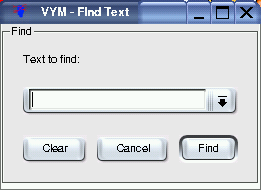
\includegraphics[width=6cm,bb = 0 0 200 100, draft, type=eps]{images/find-window.png} 
\par\end{center}

La fonction va rechercher le texte dans toutes les branches et dans
les notes associées. À chaque fois que vous appuyez sur le bouton
\og Find \fg{} il va rechercher la prochaine occurrence qui est
sélectionnée automatiquement. Si la recherche échoue, un court mess
sage \og Nothing found \fg{} (rien trouvé) va apparaître en bas
dans la {\em barre de status} du mapeditor.


\subsubsection*{\label{hideunselected}Garder la visibilité, cacher une partie de
la carte}

Une très grande arborescence (une branche avec une centaine d'enfants
par exemple) rend difficile la vue d'ensemble de la carte. Vous pouvez
cacher les enfants en les {\em enroulant}. Cette fonction est souvent
appelée {\em escamotage} (folding). Pensez que tout le sous-arbre
est dessiné sur un rouleau de papier. Vous pouvez le dérouler ou l'enrouler
pour ne voir que la première ligne.

Pour escamoter ou ré-afficher une branche et ses fils vous pouvez
au choix : 
\begin{itemize}
\item appuyez sur \key{Scroll Lock} ou \key{S},
\item appuyer sur le bouton milieu de la souris,
\item choisir l'icône sur le menu de travail.
\end{itemize}
Si vous sélectionnez une branche cachée --par la fonction de recherche
ou en utilisant les flèches de direction par exemple-- elle va devenir
provisoirement visible. Cela est montré comme un défilement avec une
petite loupe. Si la partie \og dé-cachée \fg{} n'est plus nécessaire,
elle est de nouveau cachée automatiquement. Il est possible de rendre
toutes les branches visibles en utilisant le menu \og Edit\ra Unscroll
all scrolled branches \fg{}.

Vous pouvez cacher des parties de la carte pour l'exporter dans une
page web ou pour une présentation par exemple voir \ref{hideexport}
pour plus de détails.


\subsection{Modifier et déplacer les branches}


\subsubsection*{Modifier le titre}

On peut éditer le titre en sélectionnant la branche puis au choix
:
\begin{itemize}
\item appuyer sur \key{Enter} 
\item ou \key{F2} 
\item faire un double clic avec le bouton gauche de la souris.
\end{itemize}
Écrivez votre nouveau titre (ou éditez le) puis appuyez sur \key{Enter}
pour valider.


\subsubsection*{Déplacer une branche}

Le moyen le plus simple de déplacer une branche est de la sélectionner
avec le bouton gauche de la souris et de la déplacer à sa destination
en maintenant le bouton enfoncé. Suivant la branche elle sera :
\begin{itemize}
\item déplacée vers la destination,
\item {\em liée } à un nouveau {\em parent} (mapcenter ou branche) 
\end{itemize}
Si vous déplacez la branche au dessus d'une autre ou du mapcenter,
vous pourrez constater que le lien le connectant à l'ancien parent
va être changé pour aller au nouveau situé sous le curseur de la souris.
Si vous relâchez alors le bouton, la branche va être reliée.

Si vous relâchez le bouton n'importe où, le résultat dépendra du type
de branche que vous déplacez :
\begin{itemize}
\item Une branche principale directement connectée au mapcenter. Il va rester
à sa nouvelle position,
\item Une autre branche \og ordinaire \fg{} va rejoindre sa position d'origine.
\end{itemize}
Vous pouvez ainsi facilement réarranger la disposition des branches
principales pour qu'elles ne recouvrent pas leurs branches filles.
Il y a un autre avantage à déplacer les branches, surtout si vous
voulez {\em réorganiser} un sous-arbre. Vous pouvez monter ou descendre
une branche par l'action suivante au choix :
\begin{itemize}
\item appuyer sur \key{Page Up} ou \key{Page Down},
\item sélectionner Edit \ra Move branch,
\item appuyer sur les icônes de la barre de menu : 
\includegraphics[width=1.5cm,bb = 0 0 200 100, draft, type=eps]{images/move-buttons.png} 
\end{itemize}
%tipp
Il y a un autre moyen de déplacer des branches : si vous appuyez sur
\key{Shift} or \key{Ctrl} en bougeant la souris, la branche va
être ajoutée au-dessus ou au-dessous de la branche sur laquelle la
souris est. Cela peut être utilisé pour classer les branches dans
une carte.


\subsection{Des couleurs et des images : utiliser le côté droit de votre cerveau}


\subsubsection*{Changer la couler d'un titre}

Vous pouvez utiliser des couleurs pour mettre plus d'informations
sur la carte par exemple mettre du rouge, du vert et d'autres couleurs
pour montrer la priorité des tâches. Pour ce faire : 
\begin{itemize}
\item utiliser le menu et choisir : Format \ra Set Color 
\item utiliser la barre de menu :


\begin{center}
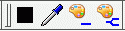
\includegraphics[width=3cm,bb = 0 0 200 100, draft, type=eps]{images/color-buttons.png} 
\par\end{center}

\end{itemize}
Le premier bouton (noir dans la figure ci-dessus) montre la couleur
courante. Cliquer dessus vous permet de choisir une autre couleur.
Vous pouvez \og piquer \fg{} la couleur d'une autre branche en la
sélectionnant et en utilisant le bouton \og pipette \fg{}. Les deux
icônes avec une palette colorent la branche sélectionnée avec la couleur
courante. Alors que la première ne colore que la sélection, la deuxième
colore tous les fils de la branche sélectionnée.

%tipp
Une autre fonction très utile est le \og copier couleur \fg{} en
utilisant la souris : sélectionner une branche qui doit avoir la nouvelle
couleur appuyez \key{Ctrl} et simultanément cliquez avec le bouton
gauche sur une autre branche pour copier sa couleur dans la branche
sélectionnée. Tout le sous-arbre sera coloré. Si vous ne voulez colorer
que la sélection appuyez sur \key{Shift} au lieu de \key{Ctrl}.


\subsubsection*{Utiliser les indicateurs}

\vym possède des indicateurs variés. Ils sont visibles dans la barre
de menu en haut de la mapeditor. (Note : Comme toutes les barres de
menu, vous pouvez les déplacer sur le côté droit ou gauche ou même
les détacher. Prenez la ligne pointillée à gauche de la barre de menu
avec le bouton gauche de la souris.) \maximage{images/default-flags.png}
Si vous avez une branche sélectionnée, vous pouvez positionner n'importe
quel indicateur en les cliquant sur la barre de menu. Les boutons
de la barre de menu changent d'état et reflètent l'état des indicateurs
de la branche sélectionnée. Ainsi pour effacer un indicateur d'une
branche, sélectionnez la branche et cliquez sur le bouton de la barre
de menu enfonce.

Pour l'instant \vym utilise deux sortes d'indicateurs : les {\em
Indicateurs Standard} et les {\em Indicateurs Système}. Les indicateurs
standard sont ceux que l'on voit dans la barre de menu. Les Indicateurs
Système sont positionnés par \vym pour indiquer qu'il y a par exemple
de l'information supplémentaire dans une note (plus d'information
dans \ref{noteeditor}). Dans des versions futures de \vym il pourra
y avoir une autre sorte d'indicateurs éditables par l'utilisateur.


\subsubsection*{Images}

Le moyen le plus simple pour ajouter une image à une branche est de
la déplaçer par exemple à partir d'un navigateur dans le mapeditor
pendant qu'elle branche est sélectionnée.

Vous pouvez aussi ajouter une image en ouvrant le menu contextuel
d'une branche. Cliquez à droite sur la branche sélectionnée, choisissez
\og Add Image \fg{}. Une fenêtre de dialogue vous permet de la choisir.%
\footnote{Les formats d'images supportés sont : PNG, BMP, XBM, XPM et PNM. Sont
aussi supportables JPEG, MNG et GIF, si spécialement configuré pendant
la compilation dans  SUSE LINUX).%
} Quand une image est sélectionnée dans le dialogue, un aperçu est
affiché. Il est possible de sélectionner plusieurs images.

Vous pouvez placer l'image où vous voulez, vous n'avez qu'à la déplacer
avec la souris en appuyant sur le bouton gauche. Pour la lier à une
autre branche, appuyer sur la touche \key{Shift} en la déplaçant.
Pour l'effacer appuyer sur la touche \key{Del}.

Si vous cliquez à droite sur une image, un menu de contexte s'ouvre
qui vous permet de sélectionner un des multiples format d'image. Puis
une fenêtre s'affiche pour sauver l'image.

\hint{On utilise cela  pour \og exporter \fg{} l'image, l'image
sera sauvegardée dans la carte elle-même. Vous pouvez aussi copier-coller
des images mais il n'est pas possible de lui ajouter des objets. Les
images sont considérées comme des \og particularités supplémentaires%
\footnote{extra feature (N.d.T.)%
} \fg{}. Elles pourraient rendre le travail avec la carte beaucoup
plus complexe par exemple en liant des images à des images.}

L'option \og Use for export \fg{} contrôle la sortie des exportations
par exemple en HTML : si positionné à NON, l'image n'apparaîtra pas
dans le {\em texte} de la sortie. C'est utile pour les grandes
images ou si des images sont utilisées comme trames comme par exemple
le nuage autour d'une partie de la carte. Elle n'apparaîtront pas
au milieu du texte.

Pour le moment le support des images est provisoire : les images sont
sauvées avec les autres données de la carte dans le fichier \texttt{.vym}.
Des versions futures incluront plus de possibilités comme le redimensionnement
des images et changer sa transparence et l'inclure dans le fond de
la carte), etc.


\subsubsection*{Trames}

Une trame peut être ajoutée à une branche dans la {\em fenêtre des
propriétés} (voir \ref{propwindow}). Vous pouvez aussi utiliser
des images comme trames. Regardez la carte de démonstration \texttt{todo.vym}
comme exemple, où le mapcenter est un nuage. Vous pouvez utiliser
un programme de dessin externe comme\texttt{ gimp} pour créer une
image, de préférence avec un canal de transparence, ainsi vous pouvez
créer des trames qui n'ont pas de bord rectangulaire, comme un nuage.


\subsection{Conception du fond des cartes et des liens de connections}

La conception du fond d'une carte et aussi des liens reliant les diverses
parties de la carte peuvent être changés par :
\begin{itemize}
\item la sélection du format à partir du menu,
\item en cliquant à droite sur le fond de la carte, ce qui ouvre un menu
de contexte.
\end{itemize}

\subsubsection*{Trame de fond}

La couleur est choisie (et aussi affichée) par \og Set background
colour \fg{}. Vous pouvez aussi choisir une image de fond d'écran
quoique cela ne soit pas recommandé. Travailler sur la carte devient
lent et l'image ne peut être positionnée librement.


\subsubsection*{Couleur des liaisons}

Les liaisons reliant les branches peuvent être colorées de deux façons
: 
\begin{itemize}
\item utiliser la même couleur pour le titre et la ligne représentant la
liaison,
\item utiliser {\em une} couleur pour toutes les liaisons et choisir
des couleurs différentes pour les titres. La couleur par défaut des
liaisons des branches est bleu.
\end{itemize}
Cette dernière couleur peut être choisie par \og Set link colour \fg{}.
Positionner ou invalider l'option \og Use colour of heading for link \fg{}
pour basculer entre deux choix dans votre dessin.


\subsubsection*{Style de liaison}

\vym offre quatre styles différents pour l'apparence des liaisons
:
\begin{itemize}
\item ligne,
\item parabole,
\item grosse ligne,
\item parabole épaisse.
\end{itemize}
Les styles \og épais \fg{} ne sont actifs que pour les liaisons
partant du mapcenter, les liaisons pour le reste de la carte sont
toujours \og fines \fg{}.


\subsection{Liens à d'autres documents et aux pages web}

\vym admet deux types de liens externes :
\begin{itemize}
\item document qui va être ouvert dans un navigateur externe,
\item carte \vym, qui sera ouverte par \vym lui-même.
\end{itemize}
En supplément aux liens externes, il y en a d'autres internes, reliant
une branche à une autre sur la même carte. Elles sont appelées {\em
XLinks} et sont expliquées à la section ~\ref{xlinks}.


\subsubsection*{navigateur}

Les navigateurs modernes comme \texttt{konqueror et Firefox} sont
capables d'afficher des types de fichiers variés locaux ou sur Internet.
Pour saisir l'~URL d'un document appuyez sur la touche \key{U}
ou cliquez à droite sur une branche pour ouvrir le menu contextuel
puis choisir \og References\ra Edit URL \fg{}. Si vous voulez ouvrir
une fenêtre de dialogue pour choisir plus facilement un fichier local
tapez ~\key{SHIFT-U}.

Lorsqu'une URL a été entrée, un petit globe apparaît dans la branche.
On cliquant sur ce globe ou dans le menu contextuel, le navigateur%
\footnote{Le navigateur peut être changé dans le menu Settings (voir \ref{settings}).%
} externe sera lancé :

\begin{center}

\includegraphics[width=0.5cm,bb = 0 0 200 100, draft, type=eps]{images/flag-url.png} 
\par\end{center}

Pour plus d'informations sur le travail avec les signets et les navigateurs
voir \ref{bookmarks}.

Dans le menu de contexte, il y a une option pour ouvrir toutes les
URL trouvées dans le sous-arbre de la branche sélectionnée. C'est
très pratique pour ouvrir tout un jeu de liens dans le navigateur
surtout si celui-ci dispose d'index (comme \texttt{konqueror}%
\footnote{ou \texttt{firefox} (N. d. T.)%
}).


\subsubsection*{carte \vym }

Pour lier une branche à une autre carte \vym  cliquer à droite sur
une branche et choisir : \og Édit \vym links \fg{}. Une fenêtre
de dialogue sur les fichiers s'ouvre pour vous permettre de choisir
le fichier voulu. Une branche avec un lien est marquée par :

\begin{center}

\includegraphics[width=0.5cm,bb = 0 0 200 100, draft, type=eps]{images/flag-vymlink.png} 
\par\end{center}

Cliquer sur cet indicateur, dans la barre de menu ou dans le menu
de contexte va ouvrir cette carte dans un autre onglet. (voir \ref{tabs}
pour le travail sur plusieurs cartes). Pour effacer un lien existant,
cliquer à droite sur la branche et choisir \og Delete \vym link \fg{}.

Dans le menu contextuel, il y a aussi une option pour ouvrir tous
les liens vers des fichiers \vym  du sous-arbre de la branche sélectionnée
dans la carte. C'est utile pour ouvrir simultanément une collection
de cartes en relation avec la carte courante.

Note technique : en interne \vym utilise des chemins absolus, pour
éviter d'ouvrir plusieurs fois la même carte. Quand la carte est sauvegardée,
le chemin est converti en relatif (par exemple \texttt{/home/user/vym.map}
devient\texttt{ ./vym.map}. Cela rend aisé d'utiliser des cartes différentes
sur plusieurs ordinateurs et de les exporter en HTML pour plus tard.


\subsection{cartes multiples}

\label{tabs} Vous pouvez travailler sur plusieurs cartes en même
temps. Chaque nouvelle carte est ouverte dans un {\em onglet}.
Les onglets des cartes disponibles sont situés en haut du mapeditor.
Vous pouvez utiliser les fonctions couper-copier-coller pour transférer
des données d'une carte à l'autre.

%todo


%TODO
%\subsubsection{Menus}
%\subsubsection{Keyboard shortcuts}


% Settings
% Images
% Copy & Paste
% Working with tabs (multiple maps)
% Exporting
% Scrolling



\section{Noteeditor}

\label{noteeditor}Si vous voulez mettre plus de texte sur une branche
(par exemple un email complet ou une recette de cuisine ou une palanquée
de code source) vous pouvez utiliser le noteeditor. \maximage{images/noteeditor_fr.png}
Cet éditeur affiche le texte associé à la branche sélectionnée dans
le mapeditor. 


\subsection{États}

Avant de pouvoir écrire ou mettre du texte dans le noteeditor, vous
devez sélectionner une branche dans le mapeditor. La couleur du fond
du noteeditor indique son état : 
\begin{itemize}
\item gris : pas de texte,
\item blanc : du texte existe.
\end{itemize}
Dans le mapeditor, pour signaler qu'il y a une note avec plus d'informations
pour une branche particulière, un petit indicateur \og note \fg{}
apparaît dans l'entête de la branche. Regardez dans la branche en
bas à droite de la carte suivante :\maximage{images/branches-flags_fr.png}


\subsection{Importer et exporter des notes }

Une note est automatiquement sauvée dans la carte \vym. Il est agréable
d'importer une note à partir d'un fichier externe ou d'écrire cette
note dans un fichier externe. Dans le noteeditor utiliser \og File\ra~Import \fg{}
et \og File\ra~Export \fg{} pour l'import-export.


\subsection{Éditer et imprimer une note}

L'édition fonctionne comme un éditeur de texte classique, incluant
les fonctions annule-recommence. Vous pouvez effacer entièrement la
note en cliquant sur la corbeille. En cliquant sur le bouton d'impression
seule la note et imprimée.


\subsection{RichText: couleurs, paragraphes et texte formatté}

\vym supporte le texte formatté (QT Rich Text) dans le noteeditor
depuis la version 1.4.7. Les couleurs et les attributs de texte (par
exemple italique, gras) sont positionnés avec les boutons au-dessus
du texte. Le texte lui-même est divisé en paragraphes. Pour chaque
paragraphe l'alignement peut être spécifié (par exemple centré ou
à droite). Un paragraphe est terminé par appui sur la touche \key{Return}.
Si vous voulez juste commencer une nouvelle ligne tapez \key{CTRL-Return}.


\subsection{Les fontes et comment les changer rapidement}

Le noteeditor est fait pour éditer de petites notes, ce n'est pas
un traitement de texte complet. Suite à beaucoup de demandes, \vym
supporte le texte formatté dans le noteeditor%
\footnote{\vym utilise le format QRichtText, qui est un sous-ensemble du formattage
fourni en HTML.%
}. Deux fontes par défaut sont installées qui peuvent être choisies
par le \og Settings menu \fg{} (voir \ref{settings}). Une fonte
à chasse fixe, l'autre variable. La fonte à chasse fixe est utilisée
pour les emails, le code source, etc l'autre pour les simples notes.
Les deux fontes peuvent être facilement commutées en cliquant sur
le bouton suivant dans la barre de menu :

\begin{center}

\includegraphics[width=0.5cm,bb = 0 0 200 100, draft, type=eps]{images/formatfixedfont.png} 
\par\end{center}

Dans le \og Settings menu \fg{} les deux fontes peuvent être choisies.
La fonte par défaut peut aussi être changée en sélectionnant ou désélectionnant
\og fixed font is default \fg{}.

En supplément toute fonte installée sur votre système peut être utilisée.
Notez que la fonte choisie sera aussi utilisée pour les exports HTML,
si vous voulez exporter votre carte \vym  l'intranet ou sur le web,
vous devrez utiliser des fontes disponibles partout.


\subsection{Recherche de texte}

Le noteeditor n'a pas sa propre fonction de recherche, utiliser \og Find \fg{}
dans le mapeditor qui recherche également dans toutes les notes (voir
\ref{findwindow}).


\subsection{Coller du texte dans le noteeditor}

Vous voulez souvent coller du texte dans le noteeditor à partir d'une
autre application par exemple un email. Normalement \vym va créer
un nouveau paragraphe pour chaque ligne. Si ce n'est pas ce que voulez
vous pouvez choisir à partir de la barre de menu


\section{Hello world%
\footnote{\og bonjour monde \fg{} ou comment faire une carte de base%
}}

Cette section décrit comment \vym réagit au contact d'autres applications.
Maintenant beaucoup d'applications lisent et écrivent leurs données
en XML, le \og eXtensible Markup Language \fg{}. \vym utilise aussi
XML pour sauver ses cartes, voir \ref{fileformat} pour une description
plus détaillée.

Si vous utilisez une autre application qui utilise le XML, il est
possible de faire un filtre d'import-export pour \vym. Les volontaires
sont accueillis avec plaisir ;-)


\subsection{Import}

\label{import}


\subsubsection*{Signets KDE }

L'éditeur de signets intégrés à KDE (Konqueror etc.) est limité, ainsi
pourquoi ne pas utiliser \vym pour gérer les signets? Pour créer
une nouvelle carte contenant contenant les signets courants choisir
: \og File \ra Import\ra KDE Bookmarks \fg{}


\subsubsection*{Mind Manager}

\vym a pour l'instant un filtre d'importation rudimentaire pour convertir
les cartes créées par {\em Mind Manager}%
\footnote{Mind Manager est un logiciel commercial c'est à dire non libre. Il
est développée par Mindjet pour Windows et le Mac. Les deux sont des
marques enregistrées par Mindjet. Pour plus d'informations voir leur
site web \href{http://mindjet.com}{http://mindjet.com}%
} en cartes \vym. Les notes et les images ne sont pas converties pour
l'instant. Vous pouvez importer des fichiers avec : \og File \ra
Import\ra Mind Manager \fg{}.


\subsubsection*{Structure et répertoires}

\vym peut lire une structure de répertoires. C'est pour tester \vym,
par exemple pour créer facilement de très grandes cartes utilisées
pour les essais (oui il y a encore de la place pour optimiser \vym
;-)


\subsection{Export}

\label{export} \label{hideexport} Souvent vous ne voulez pas exporter
la carte entière, juste une partie. Par exemple, vous pouvez avoir
une information supplémentaire dont vous voulez parler dans une présentation,
alors que ces parties ne seront pas visibles pendant la présentation.
Pour y arriver, vous pouvez \og cacher \fg{} des parties de la carte
pendant les exports en positionnant l'indicateur \og hide in export \fg{}. 

\begin{center}

\includegraphics[width=0.5cm,bb = 0 0 200 100, draft, type=eps]{images/flag-hideexport.png} 
\par\end{center}

Vous pouvez basculer cet indicateur à partir de la barre de menu ou
en tapant \key{H}. Notez qu'il y a une option globale dans le menu
de préférences( \ref{settings}) pour basculer l'utilisation de cet
indicateur. Par défaut cet indicateur est validé.


\subsubsection*{Open Office}

À partir de la version 2 Open utilise le \og Open Document Format \fg{},
qui peut être écrit par \vym. Les options sont actuellement limitées.
Il est possible d'exporter des présentations qui peuvent être ouvertes
par Open Office Impress. En sélectionnant : \og File \ra Export\ra
Open Office \fg{}.

Vous obtenez une fenêtre de dialogue où vous pouvez choisir le fichier
de sortie et le type de fichier : \maximage{images/export-oo.png}
Les types de fichiers représentent différents types de patrons, qui
peuvent être créés à partir d'un document Open Office avec un peu
de travail manuel. La structure de la carte \vym est alors insérée
dans ce patron. Il y a pour l'instant quelque limitations :
\begin{itemize}
\item \vym ne peut gérer la longueur des pages, vous devez tester et sans
doute re-éditer le document Open Office pour éviter que le texte ne
continue après la fin de la page,
\item images et les indicateurs ne sont pas utilisés pour le moment,
\item les notes sont écrites en texte brut , sans RichText 
\item la gamme complète des patrons n'est pas disponible dans toutes les
distributions.
\end{itemize}
Certains patrons utilisent des {\em sections} c'est à dire qu'ils
insèrent le titre des branches principales comme des titres de section
dans la présentation.


\subsubsection*{Image}

\vym supporte tous les formats d'image qui sont nativement supportés
par le QT~toolkit : BMP, JPEG, PBM, PGM, PNG, PPN, XPM et XBM. Pour
utilisation sur les sites web ou envoyer des images par email, PNG
est un bon compromis taille/qualité. \vym utilise les options par
défaut de Qt pour comprimer les images.


\subsubsection*{ASCII}

L'exportation en image est expérimental en ce moment. Plus tard cela
sans doute fait avec des feuilles de style. La forme de la sortie
risque de changer dans de futures versions de \vym.


\subsubsection*{\protect\LaTeX{}}

\vym peut générer un fichier d'entrée pour \LaTeX{}. C'est actuellement
en développement, il n'y a pas d'option. En sélectionnant : \og File
\ra Export\ra \LaTeX{} \fg{}.

Vous allez ouvrir une fenêtre de dialogue pour le nom du fichier de
sortie. Cette feuille peut ensuite être inclue dans un document en
utilisant la commande : \begin{verbatim} \include{inputfile} \end{verbatim}


\subsubsection*{Bookmarks KDE }

\vym va écraser le fichier des bookmarks KDE puis tenter de le notifier
à Konqueror en fonctionnement puis essayera de le notifier via DCOP
que le fichier a changé. \emph{\vym ne crée pas de sauvegarde ! } Accessible
par le menu : \og File \ra Export \ra KDE Bookmarks \fg{}.


\subsubsection*{XHTML (Webpages)}

C'est le format à utiliser si vous voulez créer une page web. Pour
voir un exemple visitez la page d'entrée de \vym : \href{http://www.InSilmaril.de/vym}{www.InSilmaril.de/vym}

Quelque explications sur son fonctionnement : avant d'exporter une
carte en XHTML, elle est d'abord écrite en XML dans un répertoire
(voir \ref{xmlexport}). Puis le programme externe \texttt{xsltproc}%
\footnote{Sur la distribution SUSE Linux et quelques autres distributions \texttt{xsltproc}
est installé par défaut.%
} va être appelé pour traiter le fichier XML et générer le code HTML.
Un dialogue permet à l'utilisateur de positionner diverses options
:
\begin{description}
\item [{Include}] \textbf{image:} si positionné, \vym va créer une une
image de la carte au début de la sortie HTML. Cliquer sur une branche
va faire sauter à la section correspondante de la sortie.
\item [{Colored}] \textbf{headings:} Si positionné à OUI, \vym va mettre
les titres en couleur dans la partie texte avec les mêmes couleurs
que celles utilisées dans la carte \vym. 
\item [{Show}] \textbf{warnings:} Si positionné, \vym va demander avant
d'écrire les données.
\item [{Show}] \textbf{output:} Cela est utilisé principalement pour le
dégogage. On va voir comment s'effectue le traitement du fichier XML
en appelant le programme externe \texttt{xsltproc}. 
\end{description}
En complément les chemins des feuilles de styles CSS et XSL peuvent
être indiqués. Par défaut sur SUSE~Linux elles sont dans : \texttt{/usr/share/vym/styles}%
\footnote{N.dT. idem pour la version 1.10.0 sur Debian Etch%
}.


\subsubsection*{XML}

\label{xmlexport} La carte est écrite dans un répertoire à la fois
comme une image et comme un fichier XML. Le répertoire est choisi
dans une fenêtre de dialogue. Si le répertoire n'est pas vide, vous
allez être averti et on va vous prévenir que vous risquez d'écraser
des fichiers.

Il est possible d'exporter des cartes différentes dans le même répertoire.
Chaque fichier généré va avoir le nom de la carte comme préfixe, par
exemple e.g. \texttt{todo.vym} devient \texttt{todo.xml}, \texttt{todo.png},
\texttt{todo-image-1.png} et ainsi de suite. C'est utile si par exemple
un site web comporte des cartes liées qui doivent être rangées dans
le même répertoire.


\subsubsection*{Export d'une partie d'une carte}

Sélectionnez la branche que vous voulez exporter avec ses fils, puis
ouvrez le menu contextuel et choisissez {\em Save Selection}. Cela
va créer un fichier avec le suffixe \texttt{.vyp}, qui est une abréviation
de \og vym part \fg{}.


\section{Édition avancée}


\subsection{Propriétés d'un objet}

Pour chacune des branches vous pouvez ouvrir une fenêtre auxiliaire
(voir \ref{satellite}): la {\em property window%
\footnote{fenêtre des propriétés%
}}: 

\begin{center}
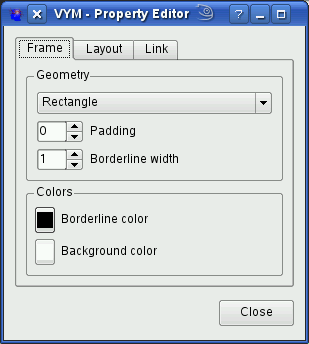
\includegraphics[width=8cm,bb = 0 0 200 100, draft, type=eps]{images/propwindow.png}
\label{propwindow} 
\par\end{center}

%FIXME create screenshot
%FIXME explain the tabs

\begin{itemize}
\item trame,
\item lien (voir \ref{hideunselected}) 
\item Layout (voir \ref{incimg}) 
\end{itemize}

\subsection{Revoir l'histoire : défaire et refaire %
\footnote{Undo and Redo%
}}

\vym garde la trace de tous les changements faits à une carte. Le
nombre de modifications qui peuvent être défaites est de 75 par défaut.
L'historique complet peut être vu dans la {\em fenêtre d'historique}:
\maximage{images/historywindow.png} \label{historywindow} un simple
pas en arrière peut être défait ou refait en tapant \key{CTRL-Z}
ou \key{CTRL-Y}, ou en utilisant les boutons de la barre de menu
ou la {\em fenêtre d'historique}. Dans la {\em fenêtre d'historique},
vous pouvez cliquer sur une ligne pour détailler toutes les actions
faites jusqu'à ce moment, ou refaire toutes les actions en cliquant
sur la dernière ligne.

\hint{ Vous pouvez \og coller à partir du passé \fg{} : aller en
arrière dans le temps avec la touche \key{CTRL-Z}, puis copier dans
le tampon en tapant \key{CTRL-C}.

Maintenant pour refaire toutes les actions, par exemple en tapant
sur la touche \key{CTRL-Y} ou en cliquant sur la dernière action
dans la {\em fenêtre d'historique}. Maintenant collez à partir
du passé avec la touche \key{CTRL-V}. }


\subsection{Macros}

\label{macros} Les macros ont été ajoutées à \vym à la version~1.9.0.
Jusqu'à présent elles sont provisoires, elles vont peut-être être
remplacées par un langage de script plus performant (les commandes
seront approximativement les mêmes).

Chaque touche de fonction (touches \key{F1} à \key{F12}) contient
une macro, qui est exécutée sur la sélection courante lorsque la touche
est enfoncée. Les macros par défaut changent la couleur d'un sous
arbre ou positionnent la trame d'une branche : 

\begin{center}
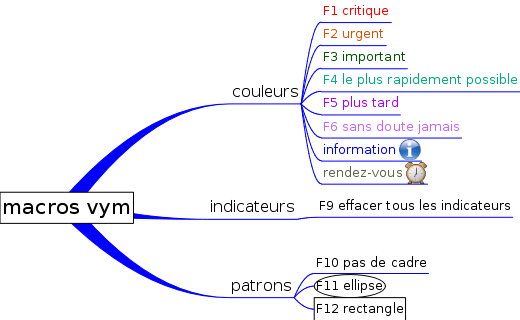
\includegraphics[width=8cm,bb = 0 0 200 100, draft, type=eps]{images/macros_fr.png} 
\par\end{center}

Chaque macro est un script \vym qui est exécuté lorsque la touche
correspondante est appuyée. L'emplacement par défaut des macros peut
être changé dans le \og Settings menu \fg{}. Plus d'informations
sur l'utilisation des scripts dans \vym peut être trouvé en appendice~\ref{scripts}.


\subsection{Signets}

\label{bookmarks} 


\subsubsection*{Ouvrir des nouveaux signets au lieu de nouvelles fenêtres}

Si vous utilisez \texttt{konqueror} comme navigateur, \vym peut se
rappeler de la session de \texttt{konqueror }qui était ouverte en
premier par \vym. Vous pouvez appuyer sur les touches \key{Ctrl}
et cliquer pour ouvrir le lien dans un nouvel onglet.

\vym peut aussi ouvrir une nouvel onglet dans Mozilla ou Firefox
en utilisant la commande à distance %
\footnote{(remote command) à \href{http://www.mozilla.org/unix/remote.html}{http://www.mozilla.org/unix/remote.html}%
} de ces navigateurs.


\subsubsection*{Copier/coller}

Si vous voulez mettre vos bookmarks dans une carte, sélectionnez une
branche où vous voulez ajouter le bookmark, puis collez simplement
l'URL dans la carte à partir de votre navigateur. Vous pouvez aussi
utiliser un titre existant comme URL : cliquez à droite sur la branche
et sélectionnez : \og Use heading for URL \fg{}.


\subsubsection*{Accès direct à la liste des bookmarks d'un navigateur}

Voir les sections \ref{import} et \ref{export} sur les filtres d'import-export.


\subsubsection*{URL spéciales}

\vym peut convertir un titre d'une branche existante en URL. Cela
marche pour Bugentries dans le système Novell Bugtracking : ouvrez
le menu de contexte d'une branche (en cliquant à droite) et sélectionnez
: \og Create URL to Bugzilla \fg{}.

L'URL sera créé à partir du titre.


\subsection{Associer des images à une branche}

\label{incimg} La configuration par défaut d'une image est de flotter
\og librement \fg{}. Les images peuvent être positionnées n'importe
où dans le canevas cachant la partie correspondante de la carte.

La solution est de l'insérer ou de l'inclure \og dans \fg{} une
branche. Cela est fait au travers de la fenêtre de propriétés (voir
\ref{propwindow}) par les menus : 
\begin{itemize}
\item include images horizontally 
\item include images vertically 
\end{itemize}
L'images est positionnée relativement à sa branche mère, mais le titre
et la bordure s'adapte à l'image flottante, voir en dessous : \maximage{images/includeImages_fr.png}


\subsection{Mode modificateur}

Les modificateurs sont par exemple la touche \key{Shift}, \key{Ctrl}
ou \key{Alt}. Quand on appuie dessus pendant une action de la souris,
\vym va effectuer une action différente de celle habituelle.

%\key{Ctrl} or \key{Alt}is pressed while releasing the branch, it will be
%added above/below the target, not as child of the target.


Sans appuyer sur un modificateur, le premier clic sur la souris sélectionne
une branche. Le comportement avec le modificateur \key{Ctrl} est
sujet à à plusieurs options, qui peuvent être positionnées dans la
barre de menu :

\begin{center}
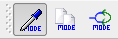
\includegraphics[width=3cm,bb = 0 0 200 100, draft, type=eps]{images/modmodes.png} 
\par\end{center}

Le mode par défaut est de copier la couleur de la branche cliquée
vers la branche sélectionnée. La figure au-dessus montre la barre
de menu avec le modificateur par défaut sélectionné. Le deuxième modificateur
vous permet de couper une branche complète avec un simple clic. Le
troisième modificateur vous permet de créer des liens entre branches
appelés {\em xLinks}. Cela est expliqué dans la section suivante
\ref{xlinks}.


\subsection{Cacher les liens d'objets non sélectionnés}

\label{hidelink} Il est pratique de positionner librement une branche,
comme une branche principale ou une image. Cela est possible pour
toutes les branches, vous pouvez utiliser une branche principale et
cacher ses liens de connexion au centre de la carte ou cacher le lien
entre une branche fils et son parent. C'est utile par exemple pour
les légendes ou pour une collection de liens \vym  pointant vers
d'autres cartes : 

\begin{center}
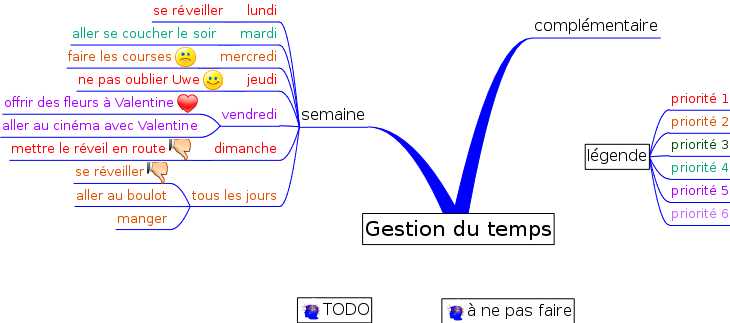
\includegraphics[width=9cm,bb = 0 0 200 100, draft, type=eps]{images/hiddenlink_fr.png} 
\par\end{center}

Pour cacher le lien entre la branche et son parent ouvrir la fenêtre
de propriétés et sélectionner \og Hide link if object is not selected \fg{}
sur l'onglet \og Link \fg{}.


\subsection{XLinks}

\label{xlinks} Jusqu'à maintenant les données dans la carte \vym
étaient sous forme d'arbre. En utilisant les xLinks vous pouvez lier
une branche à n'importe quelle autre, comme en attachant une corde
entre deux branches dans un vrai arbre. C'est très pratique dans des
cartes compliquées, où vous avez des renvois qui ne peuvent être affichés
dans la même zone visible de la fenêtre du {\em mapeditor}. La
carte suivante tient sur un écran, mais montre comment les données
peuvent être reliées. Dans le graphisme il y a un lien à partir d'une
tâche (prepare a presentation) à l'information générale : \maximage{images/xlink_fr.png}
Notez qu'un xLink qui pointe sur une branche non visible (parce qu'elle
est \og enroulée \fg{}), est montrée par une flèche horizontale.
Regardez la branche \lq Tuesday\rq dans la capture d'écran ci-dessus.


\subsubsection*{Créer un xLink}

Choisir le type de lien à partir de la barre de modifier (en cliquant
l'icône de la barre de menu ou en tapant \key{L}). Sélectionner
la branche d'où le xLink doit partir. Appuyer sur le modifier \key{Ctrl}
puis cliquez la branche et amenez le curseur de la souris où le lien
doit se terminer. Un lien est tracé qui suit le pointeur de la souris.
Le lien devient permanent quand vous relâchez le bouton de la souris
.


\subsubsection*{Modifier ou effacer un xLink}

Sélectionner une extrémité du xLink. Ouvrir le menu contextuel et
sélectionnez \og  Edit xLink \fg{}. Un sous menu contenant tous
les xLinks de la branche apparaît. Sélectionnez en un et la fenêtre
de dialogue xLink dialogue s'ouvre, où vous pouvez sélectionner la
couleur, la largeur et aussi effacer le xLink.


\subsubsection*{Suivre un xLink}

Dans une carte \vym compliquée il est commode de sauter à l'autre
extrémité d'un xLink. Vous pouvez le faire en ouvrant le menu contextuel
et en cliquant \og  Goto xLink \fg{} puis en sélectionnant le xLink
qui vous intéresse.


\subsection{Ajouter et supprimer des branches}

Le menu contextuel d'une branche montre quelques moyens supplémentaires
pour ajouter ou supprimer des données. Vous pouvez supprimer une branche
tout en gardant ses enfants. Les enfants sont alors liés au parent
de la branche supprimée (son \og grand-parent \fg{}). Des branches
identiques peuvent être ajoutées à des cartes existantes. Pour les
raccourcis clavier regarder également dans le menu contextuel.


\subsection{Ajouter une carte complète ou une partie}

Sélectionner la branche où vous voulez ajouter une carte sauvée précédemment
(\texttt{.vym}) ou une partie de carte (\texttt{.vyp}), puis ouvrez
le menu contextuel et choisissez {\em Add \ra Add Map (Insert)}.
Pour l'importation vous pouvez choisir entre {\em Add Map (Insert)}
ou {\em Add Map (Replace)}: les données importées vont être ajoutées
à la branche sélectionnée.


\section{\vym sur Mac OS X}


\subsection{Vue d'ensemble}

Il y a deux moyens de faire fonctionner \vym sur les Macs : 


\subsubsection*{Qt Mac Edition:}

\vym a là une l'apparence bien connue de Mac. \vym est disponible
comme paquet d'application Mac OS X dans une image disque (\texttt{vym.dmg}).
Il a été compilé et testé sur Mac~OS~10.4. Ce paquet inclut les
librairies Qt de Trolltech.


\subsubsection*{version X11 }

\vym peut aussi être lancé dans sa version Linux, mais les menus
et l'utilisation seront ceux de Linux c'est à dire que les barres
de menu sont différentes.


\subsection{Menu de contexte et touches spéciales}

La majorité des Macs n'a malheureusement qu'un bouton de souris. Pour
pour voir le menu contextuel qui normalement est ouvert avec un clic
droit, vous devez cliquer en appuyant sur la touche \key{command}.

Surtout sur les portables quelques touches utilisées sur les PC sont
manquantes. La version de \vym avec QT-Mac a ses propres raccourcis
clavier. Pour les trouver regardez les entrées des menus, les raccourcis
visibles à côté de cette entrée. Les boutons de la barre de menu peuvent
aussi avoir des raccourcis, positionnez le curseur de la souris sur
un bouton et la fenêtre d'aide apparaîtra.


\subsection{Voir des liens externes}

\vym sur Mac utilise le système d'appel \texttt{/usr/bin/open} pour
voir les liens. Mac~OS détermine automatiquement si le lien est un
pdf ou une page web et ouvre le bon visionneur.

\appendix \newpage{}


\section{\label{settings}\vym : processus d'initialisation et de configuration}


\subsection{Menu des préférences (Settings menu)}

Le {\em Menu des préférences } vous permet de configurer \vym
suivant vos besoins :


\subsubsection*{Choisir l'application pour ouvrir les fichiers PDF }

Choisir un visionneur PDF installé sur votre système.


\subsubsection*{Choisir le navigateur (vers les liens externes)}

Choisissez votre navigateur favori.


\subsubsection*{Positionner le chemin pour les macros}

Le chemin par défaut pour exécuter les macros correspondantes quand
vous appuyez sur une des touches de fonction. Chaque touche correspond
à un fichier (\texttt{macro-1.vys..macro12.vys}) dans le chemin de
recherche.


\subsubsection*{Niveaux défaire/refaire}

Fixer le nombre de défaire/refaire. Par défaut :75.


\subsubsection*{Sauvegarde automatique et temps entre sauvegardes}

La sauvegarde automatique des cartes peut être désactivée. Le temps
entre sauvegardes est indiqué en secondes. 

Quand la sauvegarde d'une carte est demandée \texttt{example.vym},
\vym  renomme le fichier existant en \texttt{example.vym\textasciitilde{}}
avant d'écrire le fichier \texttt{example.vym.}


\subsubsection*{Éditer la branche après l'avoir créée}

Si positionné, le titre de la nouvelle branche va être édité immédiatement
après avoir été créé.


\subsubsection*{Sélectionner la branche après l'avoir créé}

Si positionné, la nouvelle branche va être sélectionnée après avoir
été créée. Quand vous réfléchissez sur un mot donné, vous ne voulez
pas aller dans les détails, mais garder l'attention sur ce mot. Le
choix par défaut est de {\em ne pas}  sélectionner la nouvelle branche
créée.


\subsubsection*{Sélectionner la branche existante}

Si positionné et que vous commencez à éditer le titre de la branche,
le texte du titre va être sélectionné. Pratique pour copier/coller
dans d'autres applications.


\subsubsection*{Touche effacement}

Si positionné, la touche \key{Delete} est validée pour détruire
les objets. Attention aux confusions avec la touche \key{Insert}sur
les claviers de PC.


\subsubsection*{Indicateurs exclusif}

Si positionné quelques indicateurs peuvent être exclusifs, par exemple
les émoticons.


\subsubsection*{Autoriser l'indicateur caché}

Si positionné, chaque branche qui a l'indicateur caché associé (voir
\ref{hideexport}) ne sera pas présente dans les exports.


\subsection{Fichier de configuration}

Au démarrage, \vym va regarder un fichier de configuration spécifique
à l'utilisateur contenant ses réglages personnels comme la position
des fenêtres, les menus de travail, etc. Si ce fichier n'existe pas,
il sera créé. Le fichier est localisé dans la racine du répertoire
de l'utilisateur. Sa position exacte dépend de la plate-forme :

\begin{center}
\begin{tabular}{cl}
\textbf{Plate-forme}  & \textbf{Fichier de configuration }\tabularnewline
\hline 
Linux  & \texttt{$\sim$/.config/InSilmaril/vym.conf}  \tabularnewline
Mac OS X  & \texttt{/Users/NAME/Library/Preferences/com.insilmaril.vym.plist}
 \tabularnewline
\end{tabular}
\par\end{center}

Le fichier peut être édité manuellement ou sur Mac~OS~X avec le
Property List Editor (installé avec xtools).


\subsection{Chemin vers les ressources}

\vym va essayer de trouver ses ressources (images, feuilles de style,
filtres, etc) aux endroits suivants :
\begin{enumerate}
\item chemin donné par la variable d'environnement\texttt{ VYMHOME}. 
\item Si appelé avec l'option {\em local}  (voir \ref{options} en dessous),
\vym va chercher ses ressource dans le répertoire courant.
\item \texttt{/usr/share/vym} 
\item \texttt{/usr/local/share/vym} 
\end{enumerate}

\subsection{Options de la ligne de commande}

\label{options} \vym a les options suivantes lors de l'appel en
ligne de commande%
\footnote{chaque option doit être précédé du \og - \fg{} classique (N.d.T.)%
} :

\begin{center}
\begin{tabular}{cccp{8cm}}
 &  &  & \tabularnewline
\textbf{Option } & \textbf{Résumé } & \textbf{Argument } & \textbf{Description }\tabularnewline
\hline 
v  & version  &  & indiquer la version et le nom de code de \vym\tabularnewline
l  & local  &  & Utiliser les chemins locaux pour les feuilles de style,les traductions,
les icônes, etc.

Pratique pour les tests\tabularnewline
h  & aide  &  & montrer l'aide\tabularnewline
r  & lancement  & fichier  & charger et lancer un script\tabularnewline
q  & quitter  &  & quitter après le démarrage. Utile pour les benchmarks.\tabularnewline
\end{tabular}
\par\end{center}

Vous pouvez aussi donner plusieurs noms de fichiers dans la ligne
de commande pour laisser \vym ouvrir plusieurs cartes à la fois.


\section{Scripts}

\label{scripts} %FIXME


TODO: désolé cette section du manuel de \vym est provisoire.


\subsection{Exemple de scripts}


\subsubsection{Exporter un jeu de cartes}

\begin{verbatim} \# Simple vym script to export images of various
maps simultanously exportImage (); \end{verbatim} Le script au-dessus
peut être utilisé pour exporter automatiquement toutes les cartes
d'un répertoire. Si le script a pour nom \texttt{export-image.vys},
appeler \vym avec\begin{verbatim} vym --quit --run export-image.vys
{*}.vym \end{verbatim}


\section{Aider \vym}

J'ai écrit personnellement 98\% du code moi-même. Aucune surprise
: \vym correspond exactement à mes besoins. Néanmoins j'encourage
tous les utilisateurs de \vym à contribuer. Peut-être pas seulement
avec des demandes d'extensions, mais aussi avec du code, de nouveaux
filtres import/export, des traductions, etc. Dans cet appendice, je
vais essayer de montrer combien il est facile de développer avec \vym.
J'attends vraiment de vos nouvelles au sujet de vos futures extensions
!


\section{Obtenir de l'aide}


\subsection*{Foire Aux Questions}

Pointer la FAQ disponible sur le site de \vym (en anglais) :

\begin{center}
\href{http://www.InSilmaril.de/vym/faq.html}{http://www.InSilmaril.de/vym/faq.html} 
\par\end{center}


\subsection*{Mailinglists}

Il y a deux mailinglists: 
\begin{itemize}
\item \texttt{vym-forum} est le forum des utilisateurs \vym pour discuter
de points divers, 
\item \texttt{vym-devel} est fait pour les gens qui veulent contribuer à
\vym. 
\end{itemize}
Vous pouvez voir les archives et vous inscrire à :

\begin{center}
\href{https://sourceforge.net/mail/?group_id=127802}{https://sourceforge.net/mail/?group\_id=127802} 
\par\end{center}


\subsection*{Contacter l'auteur}

\label{author} En premier essayer les mailinglists. Pour tout autre
problème contacter l'auteur Uwe Drechsel à :

\begin{center}
\href{mailto:vym@InSilmaril.de}{vym@InSilmaril.de} 
\par\end{center}


\section{Comment reporter un bug}

Quoique Sourceforge ait son propre système de rapport de bugs, je
préfère que vous me contactiez directement (voir \ref{author}) ou
encore mieux : vous pouvez mettre un rapport de bug dans Bugzilla,
le système de rapport de bugs de openSUSE : 

\begin{center}
\href{http://en.opensuse.org/Submit_a_bug}{http://en.opensuse.org/Submit\_a\_bug} 
\par\end{center}

Je construis \vym régulièrement pour openSUSE, vous pouvez faire
un rapport pour une autre version , même si vous utilisez un autre
système d'exploitation. N'oubliez pas de me dire lequel vous utilisez
:
\begin{itemize}
\item les manipulations exactes pour reproduire le bug,
\item la version et la date de construction de \vym (voir l'aide Help \ra
About \vym) 
\item le matériel et le système d'exploitation
\end{itemize}

\section{Compiler à partir des sources }


\subsection{Obtenir les sources}

\label{getsources} Vous pouvez trouver la dernière version de \vym
sur le site du projet :

\begin{center}
\href{https://sourceforge.net/projects/vym/}{https://sourceforge.net/projects/vym/} 
\par\end{center}

Là vous pouvez les extraire à partir à partir du dépot des source
(CVS):\\


\begin{verbatim} cvs -d:pserver:anonymous@cvs.sf.net:/cvsroot/vym
checkout code \end{verbatim}


\subsection{le toolkit Qt }

Qt est une trousse à outils C++ multiplateforme pour les GUI%
\footnote{GUI Graphical User Interface interface graphique pour l'utilisateur
(N.d.T.)%
} et le développent d'applications. Il fournit une portabilité avec
le même source sur MS~Windows, Mac~OS~X, Linux et toutes les versions
principales commerciales d'Unix. Qt est aussi disponible pour les
systèmes embarqués. Qt est un produit de la société Trolltech. Pour
plus d'informations voir :

\begin{center}
\href{http://www.trolltech.com/qt/}{www.trolltech.com/qt} 
\par\end{center}


\subsection{Compiler \vym }

Assurez vous que vous avez installé l'environnement QT proprement,
voir la documentation pour les détails. Vous devez avoir la commande
Qt\texttt{ qmake} dans votre variable d'environnement \texttt{PATH},
pusi lancez \begin{verbatim} \$ qmake $make$ make install \end{verbatim}
La dernière commande \texttt{make install} a besoin des droits root.
Elle n'est pas nécessaire si vous voulez juste tester \vym.

%\subsubsection*{Compiling \vym on Macs}
%FIXME



\subsection{format des fichiers de \vym }

\label{fileformat}Les cartes \vym ont un suffixe \texttt{\og .vym} \fg{}
et représentent une archive compressée des données. Si vous voulez
avoir une vue plus précise de la structure des données dans la carte
\og mapname.vym \fg{}, décompressez la en lançant la commande :
\begin{verbatim} \$ unzip mapname.vym \end{verbatim} Cela va créer
les répertoires \texttt{images} et\texttt{ flags} dans votre répertoire
courant et aussi la carte elle-même, normalement appelée \texttt{mapname.xml}.
La structure XML de \vym s'explique d'elle-même, jetez un \oe il
sur le fichier \texttt{mapname.xml}.

Ce fichier XML peut être chargé directement dans \vym, il n'a pas
besoin d'être compressé. Si vous voulez compresser toutes les données
vous-même faites \begin{verbatim} \$ zip -r mapname.vym . \end{verbatim}
pour compresser toutes vos données dans le répertoire courant.


\subsection{Nouvelles fonctionnalités}

Il y a beaucoup de nouvelles fonctionnalités qui sont installées dans
\vym. Avec \vym vous avez reçu un répertoire avec un bon nombre
d'exemples de cartes. Vous les trouverez en cliquant Help \ra Open~vym~example~maps.
Vous y trouverez la carte \texttt{vym-projectplan.vym}. Elle liste
une foule de choses qui seront faites dans le futur. Si vous avez
d'autres idées, contactez l'équipe de développement à \texttt{vym-devel@lists.sourceforge.net}.


\subsection{support pour de nouvelles langues}

Pour pouvoir ajouter une nouvelle langue à \vym, vous devez disposer
des sources (voir \ref{getsources}) et de l'installation de Trolltechs
QT. une partie de QT sont des outils de développement, et particulièrement
l'outil de traduction \og Linguist \fg{} qui est nécessaire.

Dans quelques distributions Linux, les outils de développement sont
un paquetage spécial, par exemple sur SUSE LINUX vous devez avoir
installé : \begin{verbatim} libqt4-devel.rpm libqt4-devel-doc.rpm
libqt4-devel-tools.rpm \end{verbatim} Si vous n'avez pas QT de base
sur votre système, vous pouvez l'obtenir à : \href{http://www.trolltech.com}{http://www.trolltech.com}
Une fois que vous êtes capable de compiler, vous pouvez traduire le
texte dans \vym  lui-même en faisant les actions suivantes :
\begin{itemize}
\item supposons que nous voulons traduire une nouvelle langue \og NEW \fg{}
au lieu de \og de \fg{} en allemand ou \og en \fg{} en anglais,
\item copier le fichier \texttt{lang/vym\_en.ts} to l\texttt{ang/vym\_NEW.ts}
(Le code lui-même contient la version anglaise),
\item ajouter \texttt{lang/vym\_NEW.ts} dans la section TRANSLATIONS de
vym.pro,
\item lancer Linguist sur \texttt{vym\_NEW.ts} et faire la traduction,
\item lancer \texttt{lrelease} pour créer \texttt{vym\_NEW.qm.}
\item faire un make install pour installer le nouveau \vym  et tester la
traduction
\end{itemize}
Si vous vous sentez courageux, vous pouvez traduire le manuel. Il
est écrit en \LaTeX{}, vous devez juste changer le fichier \texttt{/tex/vym.tex}.
(Linguist et QT ne sont pas nécessaires, mais il est utile de savoir
comment travailler avec \LaTeX{} et pdflatex pour créer le PDF.)

S'il vous plaît envoyez moi la traduction que vous avez faite. Je
peux aussi vous donner une accès de développeur au projet, si vous
voulez fournir régulièrement des traductions.


\subsection{Nouveaux filtres d'export/import }

\vym supporte des types de filtres variés. Les données peuvent être
écrites directement, insérées dans des patrons ou peuvent être écrites
en données XML et  ensuite être travaillées par des transformations
XSL.

La plupart des fonctionnalités d'import-export est disponible dans
les classes ImportBase, ExportBase et les classes dérivées. Le tout
se trouve dans \texttt{les fichiers imports.h} et \texttt{exports.h}.


\subsection*{import/export direct}

Un exemple pour l'export direct est l'export XML. Cette méthode touche
l'implémentation de pratiquement tous les objets de \vym, aussi autant
que possible utilisez une transformation XSL à la place.

Si vous voulez savoir comment cela est fait, commencez à regarder
\texttt{MapEditor::saveToDir} in \texttt{mapeditor.cpp}.


\subsection*{patrons}

Les patrons ont été introduits pour exporter dans le format opendoc
utilisé par Open~Office. Pendant que je lisais la spécification du
format (plus de 500 pages),%
\footnote{ \href{http://www.oasis-open.org/}{http://www.oasis-open.org/}%
} j'avais le sentiment que je ne voulais pas écrire l'export à partir
de rien. Cela serait trop difficile pour adapter les styles à vos
propres besoins par exemple le canevas.

En analysant un document Open~Office existant, je trouvais qu'il
y avait un grand nombre d'informations redondantes dans une présentation
standard, par exemple chaque Item d'une liste est contenu dans sa
propre liste. À la fin j'en arrivai à un style de présentation par
défaut, qui peut encore être simplifié, si j'ai du temps de libre
\ldots{}

Les patrons existants sont encore en évolution, avant de développer
votre propre style contactez moi. De base les étapes suivantes sont
nécessaires pour que vous construisiez votre propre style :
\begin{enumerate}
\item créer un exemple dans Open Office. Utilisez un titre, les noms de
auteurs, les entêtes de page, etc que vous pourrez facilement piquer
dans le fichier de sortie,
\item décompressez le document Open Office dans un répertoire,
\item le fichier principal est appelé\texttt{ content.xml}. Toutes les données
sont sur une seule ligne. Vous pouvez exploser les marques XML en
utilisant le script \texttt{scripts/niceXML}, qui fait partie de la
distribution de \vym. 
\item copiez la sortie de \texttt{niceXML} dans \texttt{content-template.xml}.
\item en regardant dans le détail , vous trouverez nombre de définitions
inutilisées, par exemple les styles. Vous pouvez les effacer ou simplement
les ignorer.
\item Essayez de trouver votre titre, le nom de auteurs. \vym va remplacer
les chaînes suivantes lors de l'export :


\begin{center}
\begin{tabular}{lp{4cm}}
\texttt{<!-{}- INSERT TITLE -{}->}  & titre de la carte \tabularnewline
\texttt{<!-{}- INSERT AUTHOR-{}->}   & auteur\tabularnewline
\texttt{<!-{}- INSERT COMMENT -{}->}  & commentaire\tabularnewline
\texttt{<!-{}- INSERT PAGES-{}->}  & contenu de la carte \tabularnewline
\end{tabular}
\par\end{center}

Le contenu lui-même est généré d'une manière similaire en insérant
des listes dans \texttt{page-template}. Les remplacements suivants
sont effectues :

\begin{center}
\begin{tabular}{lp{7cm}}
\texttt{<!-{}- INSERT PAGE HEADING-{}->}  & entête de la page (branche principale ou fils, dépendant de l'utilisation
des sections) \tabularnewline
\texttt{<!-{}- INSERT LIST -{}->}   & tous les fils de la branche du dessus\tabularnewline
\end{tabular}
\par\end{center}

\end{enumerate}
Actuellement les images sont exportées et les notes vont apparaître
comme du texte sans mise au format ni couleur.


\subsection*{XSL Transformation}

\vym utilise des transformations XSL pour l'exportation (par exemple
en XHTML) et pour l'importation des données(par exemple les bookmarks
KDE). Il faut écrire un peu de code pour fournir le GUI, le reste
est fait en utilisant la feuille de style \texttt{.xsl} et en appelant
le processeur \texttt{xsltproc, }qui fait partie de libxslun, la librairie
C XSLT pour GNOME.
\end{document}
